\documentclass[border=0.4cm]{standalone}
\usepackage{amsmath,amssymb,amsfonts}
\usepackage[dvipsnames]{xcolor}
\usepackage{tikz}
\usetikzlibrary{arrows.meta}
\usetikzlibrary{shapes.geometric}

\begin{document}
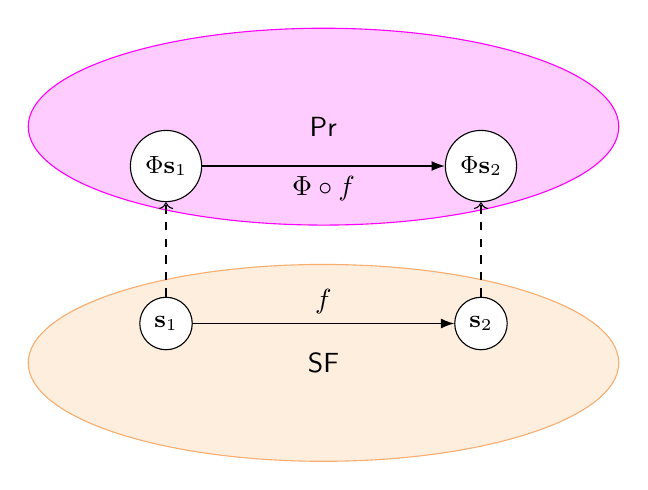
\begin{tikzpicture}
  \node[ellipse, fill=Magenta!20, draw=Magenta,
  minimum width=7.5cm,
  minimum height=2.5cm] (Pr) at (0, 2) {$\mathsf{Pr}$};
  \node[circle, fill=white, draw=black] (pr1) at (-2, 1.5) {\small$\Phi\mathbf{s}_1$};
  \node[circle, fill=white, draw=black] (pr2) at (2, 1.5) {\small$\Phi\mathbf{s}_2$};

  \node[ellipse, fill=Apricot!20, draw=Apricot,
  minimum width=7.5cm,
  minimum height=2.5cm] (SF) at (0, -1) {$\mathsf{SF}$};
  \node[circle, fill=white, draw=black] (sf1) at (-2, -0.5) {\small${\mathbf{s}_1}$};
  \node[circle, fill=white, draw=black] (sf2) at (2, -0.5) {\small${\mathbf{s}_2}$};

  \draw[->, dashed] (sf1) -- (pr1);
  \draw[->, dashed] (sf2) -- (pr2);
  \draw[-Latex] (pr1) -- node[below] {$\Phi\circ f$} (pr2);
  \draw[-Latex] (sf1) -- node[above] {$f$} (sf2);
\end{tikzpicture}
\end{document}